\section{RQ3: Stratified Profile-Coherent LightGCN}
\label{sec:rq3}

RQ2 showed that both baselines under-serve at least one risk band, with the deficit concentrated on the Conservative segment for LightGCN and on both Conservative and Income for Random Forest. RQ3 asks whether a band-aware architecture can close this gap without sacrificing ranking quality or return. We propose a profile-coherent LightGCN (PC-LightGCN) extension built from three components:
\begin{itemize}
    \item \textbf{Stratification.} A band-stratified architecture that routes each customer to a per-band sub-model.
    \item \textbf{Coherence margin.} A coherence margin added to the BPR objective.
    \item \textbf{Regrouping.} A step that reassigns customers to the band implied by their purchases.
\end{itemize}
We describe each component and the ablation setup, then evaluate the resulting configurations against the baseline LightGCN.

\subsection{Backbone}
\label{sec:method:pclgcn}
We choose LightGCN as the backbone because its differentiable loss and per-customer embeddings allow us to attach a coherence margin directly to the BPR objective. Random Forest is not extended because it ranks assets by predicted return from technical indicators alone and carries no customer-level signal to condition on.

\subsection{Stratified Architecture}
We train four band-stratified sub-models, one per declared MiFID II risk band (Figure~\ref{fig:architecture}). Each sub-model's training graph contains only the interactions of customers assigned to that band. At inference, each customer is routed to the sub-model matching their declared band. Customers with no declared band default to the Balanced sub-model.

\subsection{Profile-Coherent Margin Loss}
BPR trains the model to score an asset the customer actually bought (the positive item) higher than a randomly sampled unobserved asset (the negative item). Independently of this BPR sampling, we add a second margin term that samples one coherent asset $i_c$ (satisfying $d(u, i_c) \leq 1$) and one discordant asset $i_d$ (satisfying $d(u, i_d) > 1$) from the sub-model's asset universe, and pushes the coherent score above the discordant score:
\begin{equation}
\mathcal{L}_{\text{coh}}(u) = \text{softplus}\!\left(s(u, i_d) - s(u, i_c)\right),
\end{equation}
where $s(u, i)$ is the LightGCN inner-product score between customer $u$ and asset $i$. Here $\text{softplus}(x) = \ln(1 + e^x)$ is a smooth approximation of the hinge $\max(0, x)$: the penalty is large when the discordant asset outscores the coherent one and decays smoothly toward zero as the coherent score pulls ahead. We use softplus rather than a hard hinge because it is differentiable everywhere, giving stable gradients throughout training, and it matches the form of the standard BPR loss $-\ln\sigma(\cdot)$, keeping the two objectives consistent.

\subsection{Total Loss}
\begin{equation}
\mathcal{L} = \mathcal{L}_{\text{BPR}} + \omega \|\Theta\|_2^2 + \lambda \cdot \mathcal{L}_{\text{coh}},
\end{equation}
Here $\omega$ is the L2 weight decay on embedding parameters $\Theta$ and $\lambda \geq 0$ controls how strongly the coherence term influences training. BPR remains the primary ranking signal, and only the treatment trial activates the coherence term.

\subsection{Customer Regrouping}
\label{sec:rq3:regrouping}
The stratification and margin-loss components both condition on the customer's declared MiFID II band. RQ1 showed that this declared band is frequently inconsistent with revealed behaviour, especially at the ordinal extremes. The third component therefore \emph{regroups} customers: each banded customer is reassigned to the band implied by their revealed purchase behaviour, taken as the lower median of the risk classes of the assets they actually bought (even-count ties resolve to the more conservative band). The stratified, profile-coherent model is then retrained and routed on the regrouped bands.

\begin{figure*}[!t]
\centering
\resizebox{0.85\textwidth}{!}{%
\begin{tikzpicture}[
    >=Stealth,
    node distance=0.35cm and 0.5cm,
    box/.style={draw, rounded corners=2pt, minimum height=0.5cm,
                minimum width=1.2cm, align=center, font=\scriptsize},
    lossbox/.style={draw, rounded corners=2pt, minimum height=0.45cm,
                    minimum width=0.9cm, align=center, font=\scriptsize,
                    fill=gray!15},
    groupbox/.style={draw, dashed, rounded corners=4pt, inner sep=3pt},
    arr/.style={->, thick},
    line/.style={thick},
]

\node[box] (cust) {Customer $u$\\band $b_u$};

\node[box, right=0.5cm of cust] (router) {Band\\Router};

\coordinate (subanchor) at ($(router.east) + (1.3,0.9)$);
\node[box, anchor=west] at (subanchor) (sub0) {Cons.};
\node[box, below=0.1cm of sub0] (sub1) {Income};
\node[box, below=0.1cm of sub1] (sub2) {Balanced};
\node[box, below=0.1cm of sub2] (sub3) {Aggr.};

\node[box, right=2.0cm of $(sub1)!0.5!(sub2)$] (scores) {Scores\\$s(u, i)$};

\node[box, right=0.6cm of scores] (topk) {Top-$k$\\list};

\node[lossbox, below=0.5cm of scores, xshift=-0.6cm] (bpr) {$\mathcal{L}_{\text{BPR}}$};
\node[lossbox, below=0.5cm of scores, xshift=0.6cm] (coh) {$\lambda\!\cdot\!\mathcal{L}_{\text{coh}}$};

\draw[arr] (cust) -- (router);

\coordinate (fan-out) at ($(router.east) + (0.6,0)$);
\draw[line] (router.east) -- (fan-out);
\draw[arr] (fan-out) |- (sub0.west);
\draw[arr] (fan-out) |- (sub1.west);
\draw[arr] (fan-out) |- (sub2.west);
\draw[arr] (fan-out) |- (sub3.west);

\coordinate (fan-in) at ($(sub1.east)!0.5!(sub2.east) + (0.7,0)$);
\draw[line] (sub0.east) -- ++(0.7,0) |- (fan-in);
\draw[line] (sub1.east) -- ++(0.7,0) |- (fan-in);
\draw[line] (sub2.east) -- ++(0.7,0) |- (fan-in);
\draw[line] (sub3.east) -- ++(0.7,0) |- (fan-in);
\draw[arr] (fan-in) -- (scores.west);

\coordinate (train-split) at ($(scores.south) + (0,-0.2)$);
\draw[line] (scores.south) -- (train-split);
\draw[arr] (train-split) -| (bpr.north);
\draw[arr] (train-split) -| (coh.north);

\draw[arr] (scores.east) -- (topk.west);

\node[font=\tiny, below=0.02cm of topk.south, anchor=north] {Inference};
\node[font=\tiny, below=0.02cm of $(bpr.south)!0.5!(coh.south)$, anchor=north] {Training};

\begin{scope}[on background layer]
\node[groupbox, fit=(sub0)(sub3), label={[font=\scriptsize]above:Band-stratified LightGCN}] {};
\end{scope}

\end{tikzpicture}%
}
\caption{PC-LightGCN architecture. Each customer is routed by declared MiFID II band to a dedicated sub-model. Training combines $\mathcal{L}_{\text{BPR}}$ with a coherence margin $\lambda \cdot \mathcal{L}_{\text{coh}}$. At inference the sub-model produces the top-$k$ list directly.}
\label{fig:architecture}
\end{figure*}

\begin{table*}[!t]
\centering
\small
\begin{tabular}{lrrrrr}
\toprule
Trial & nDCG@10 & ROI@10 & Recall@10 & PC@10 & PC-lift@10 \\
\midrule
Baseline & $0.330$ & $-0.005$ & $0.495$ & $0.794$ & $1.17\times$ \\
\midrule
\textbf{Declared bands} & & & & & \\
\quad Stratify ($\lambda{=}0$) & $0.332$ & $-0.007$ & $0.501$ & $0.821$ & $1.19\times$ \\
\quad Stratify $+$ PC-loss ($\lambda{=}1$) & $0.309$ & $-0.007$ & $0.467$ & $0.918$ & $1.40\times$ \\
\midrule
\textbf{Regrouped bands} & & & & & \\
\quad Stratify ($\lambda{=}0$) & $0.352$ & $-0.006$ & $0.522$ & $0.949$ & n/a \\
\quad Stratify $+$ PC-loss ($\lambda{=}1$) & $0.333$ & $-0.005$ & $0.493$ & $0.982$ & n/a \\
\bottomrule
\end{tabular}
\caption{RQ3 aggregate metrics, averaged over 69 splits. ROI@10 is per-month. PC-lift@10 $=$ PC@10 $/\,\pi(b_u)$ and is n/a for the regrouped trials, whose shifted bands make aggregate lift incomparable (Section~\ref{sec:rq3:regroup-results}).}
\label{tab:rq4-aggregate}
\end{table*}

\subsection{Ablation and Evaluation Setup}
\label{sec:rq3:setup}
The stratified PC-LightGCN inherits the best LightGCN trial's backbone hyperparameters. Two trials run on the same 69 splits: $\lambda = 0$ trains stratified BPR alone, isolating the architecture, and $\lambda = 1$ adds the coherence margin on top.

This separates the gains from stratification and from the PC-loss, with every metric reported against the baseline LightGCN. Regrouping is evaluated by rerunning the same $\lambda \in \{0, 1\}$ ablation on the regrouped bands.

\subsection{Results}
\label{sec:rq3:results}

We read the declared-band ablation off each table and figure first, comparing the baseline against the two declared trials ($\lambda \in \{0, 1\}$). The regrouped rows and columns follow in Section~\ref{sec:rq3:regroup-results}. In Table~\ref{tab:rq4-aggregate}, the full treatment's coherence gain decomposes into a cheap stratification step and a costlier coherence-margin step.
\begin{itemize}
    \item \textbf{Full treatment ($\lambda = 1$).} Lifts PC@10 from $0.794$ to $0.918$, a $+12.4$ pp gain, and PC-lift from $1.17\times$ to $1.40\times$.
    \item \textbf{Stratification alone ($\lambda = 0$).} Supplies $+2.7$ pp of PC@10, about a quarter of the total, at virtually no cost elsewhere: nDCG@10 $+0.2$ pp, Recall@10 $+0.6$ pp, and ROI@10 $-0.2$ pp/mo, none of which registers as a meaningful effect.
    \item \textbf{Coherence margin ($\lambda = 1$).} Buys the remaining $+9.7$ pp of PC@10, roughly four-fifths of the total, at a bounded ranking cost of $-2.3$ pp nDCG@10 and $-3.4$ pp Recall@10.
    \item \textbf{ROI@10.} Essentially flat across all three trials: $-0.2$ pp/mo for stratification, $0.0$ pp/mo for the margin step alone, and $-0.2$ pp/mo for the full treatment. The small cost lives in the stratification step, not the margin, and is too small to distinguish from zero.
\end{itemize}
Together with the RQ1 coherence premium, this null ROI effect shows the recommender can be made more profile-coherent without giving up the return story.

The win rate, the fraction of splits on which a configuration beats the baseline, captures how consistently a gain is paid rather than resting on a single strong split. Looking at the win rates (Figure~\ref{fig:rq4-winrate}):
\begin{itemize}
    \item \textbf{Coherence wins everywhere.} The full treatment posts a 100\% win rate on PC@10 across all 69 splits.
    \item \textbf{Cost is uniform too.} The full treatment's nDCG@10 and Recall@10 fall below baseline on all but a handful of splits (a 7\% win rate), so the ranking penalty is a consistent shift rather than a few bad splits.
\end{itemize}

\begin{figure}[!t]
    \centering
    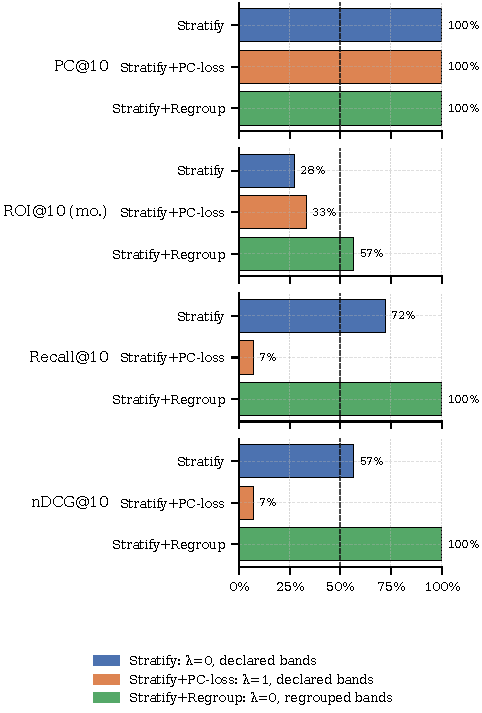
\includegraphics[width=\linewidth]{figures/paired_win_rates.pdf}
    \caption{Per-split win rates against the global LightGCN baseline for three stratified configurations: declared $\lambda{=}0$, declared $\lambda{=}1$, and regrouped $\lambda{=}0$.}
    \label{fig:rq4-winrate}
\end{figure}

Next, the paired trial-minus-baseline deltas (Figure~\ref{fig:rq4-deltas}) make each metric's shift visible split by split.
\begin{itemize}
    \item \textbf{PC@10 always positive.} PC@10 is positive on every one of the 69 splits for all three configurations, so the aggregate coherence gains are not an averaging artefact.
    \item \textbf{Ranking deltas match the table.} They track the aggregate costs from Table~\ref{tab:rq4-aggregate}: consistently negative for the declared margin trial and hugging zero for stratification alone.
\end{itemize}

\begin{figure}[!t]
    \centering
    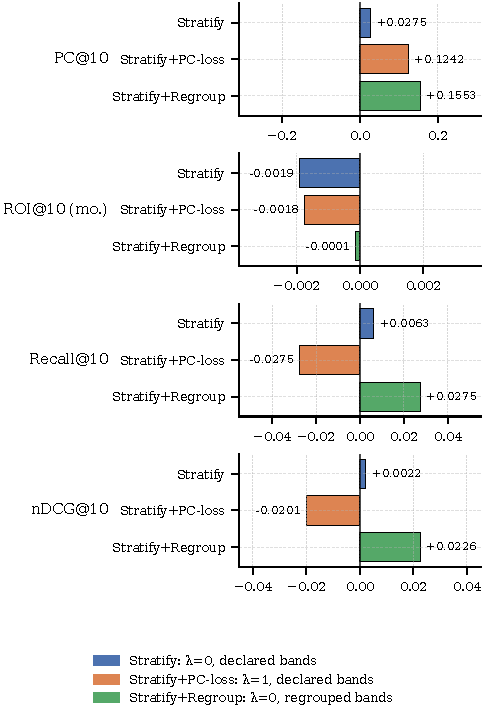
\includegraphics[width=\linewidth]{figures/paired_deltas.pdf}
    \caption{Paired per-split deltas against the baseline LightGCN for three stratified configurations: declared $\lambda{=}0$, declared $\lambda{=}1$, and regrouped $\lambda{=}0$. PC@10 is positive on every one of the 69 splits for all three.}
    \label{fig:rq4-deltas}
\end{figure}

Lastly, Table~\ref{tab:rq4-per-band} decomposes PC-lift@10 by band, tracing how the intervention resolves the per-band deficit from RQ2 (declared columns):
\begin{itemize}
    \item \textbf{Conservative.} Sits at $0.75\times$ under the baseline, climbs to $0.91\times$ under stratification alone but stays below the random baseline, and only crosses it at $1.19\times$ once the coherence margin is added.
    \item \textbf{Aggressive.} Non-monotonic: stratification alone reduces lift from $1.35\times$ to $1.17\times$, likely because the smaller Aggressive training graph yields lower-quality embeddings in isolation, but the coherence margin more than recovers the loss at $1.97\times$.
    \item \textbf{Income and Balanced.} Already above-random under the baseline, they improve modestly without being sacrificed.
\end{itemize}
Under declared $\lambda = 1$, all four bands clear the random baseline for the first time. Reading the three views together is what motivates regrouping. The coherence margin spends ranking quality to buy coherence: Figure~\ref{fig:rq4-winrate} shows nDCG@10 and Recall@10 dropping on almost every split while ROI@10 is barely touched, and Table~\ref{tab:rq4-aggregate} returns only a modest aggregate lift in return. Table~\ref{tab:rq4-per-band} shows where that cost goes: the margin is largely spent rescuing a single band, dragging Conservative from $0.91\times$ past random to $1.19\times$. Penalising incoherence during training is therefore an expensive patch for what RQ1 already flagged as noisy declared bands.

The natural alternative is to correct the labels at the source instead of fighting them with a penalty: regroup each customer onto their revealed band first, which should lift coherence under the hood.

\begin{table}[!t]
\centering
\footnotesize
\setlength{\tabcolsep}{3pt}
\begin{tabular}{lrrrrr}
\toprule
 & & \multicolumn{2}{c}{Declared} & \multicolumn{2}{c}{Regrouped} \\
\cmidrule(lr){3-4}\cmidrule(lr){5-6}
 & & Strat. & Strat.$+$PC & Strat. & Strat.$+$PC \\
Band & Baseline & $\lambda{=}0$ & $\lambda{=}1$ & $\lambda{=}0$ & $\lambda{=}1$ \\
\midrule
Conservative & $0.75\times$ & $0.91\times$ & $1.19\times$ & $1.21\times$ & $1.25\times$ \\
Income       & $1.13\times$ & $1.20\times$ & $1.26\times$ & $1.25\times$ & $1.27\times$ \\
Balanced     & $1.17\times$ & $1.22\times$ & $1.28\times$ & $1.24\times$ & $1.30\times$ \\
Aggressive   & $1.35\times$ & $1.17\times$ & $1.97\times$ & $2.24\times$ & $2.68\times$ \\
\bottomrule
\end{tabular}
\caption{Per-band PC-lift@10 for the five RQ3 configurations. Values above $1.00\times$ beat the random baseline $\pi(b)$.}
\label{tab:rq4-per-band}
\end{table}

\subsection{Effect of Regrouping}
\label{sec:rq3:regroup-results}

Rerunning the ablation on the regrouped bands changes the picture in three ways:
\begin{itemize}
    \item \textbf{Strongest and free lever.} Regrouping without the PC-loss (regrouped $\lambda = 0$) lifts PC@10 to $0.949$, a $+15.5$ pp gain that already exceeds the declared full treatment ($0.918$), and posts the highest nDCG@10 ($0.352$, $+2.2$ pp) and Recall@10 ($0.522$, $+2.7$ pp) of all five configurations with ROI@10 flat (Table~\ref{tab:rq4-aggregate}), each winning on every split (Figures~\ref{fig:rq4-winrate} and~\ref{fig:rq4-deltas}). Where the margin buys coherence by spending ranking quality, regrouping raises both together.
    \item \textbf{Dominates declared stratification.} Against declared $\lambda = 0$, it adds $+12.8$ pp PC@10, $+2.0$ pp nDCG@10, and $+2.1$ pp Recall@10 on every split and removes the small ROI cost (Table~\ref{tab:rq4-aggregate}, with the per-split wins in Figures~\ref{fig:rq4-winrate} and~\ref{fig:rq4-deltas}). Since nDCG and Recall are band-independent, this is direct evidence that the declared bands were injecting label noise.
    \item \textbf{Margin adds little once corrected.} The margin's marginal PC@10 gain collapses from $+9.7$ pp on the declared bands to $+3.3$ pp on the regrouped bands (regrouped $\lambda = 1$ reaches $0.982$), still costing $-1.9$ pp nDCG@10 and $-2.9$ pp Recall@10 (Table~\ref{tab:rq4-aggregate}). Margin and regrouping are partial substitutes, but only regrouping pays no ranking penalty.
\end{itemize}
We therefore take regrouped $\lambda = 0$ as the recommended operating point: it captures the bulk of the coherence gain at no ranking or return cost. Within the regrouped assignment every band also clears its own random baseline (Table~\ref{tab:rq4-per-band}, where regrouped $\lambda = 1$ reaches $1.25\times$ Conservative, $1.27\times$ Income, $1.30\times$ Balanced, and $2.68\times$ Aggressive).

Taken together, these results show that correcting each customer's band (regrouping) is a cheaper and stronger lever than penalising incoherence during training (the PC-loss): once the bands are corrected, it is not necessary to add the PC-loss signal during training, and because nDCG, Recall, and ROI rise alongside coherence, the declared bands rather than the model were the binding problem.

\subsection{Limitations}
\label{sec:rq3:limitations}

Two caveats bound the RQ3 results.

\begin{itemize}
    \item \textit{Single backbone and operating point.} This intervention extends only LightGCN, leaving sequential, transformer, and content-based recommenders as candidates for the same treatment, and reports a single Pareto point ($\lambda = 1$) on the inherited RQ2 best-trial hyperparameters rather than re-tuning end-to-end. The reported coherence gains are therefore a lower bound on what a full frontier sweep could achieve, and the nDCG and Recall costs an upper bound.
    \item \textit{Regrouping leakage and tautology.} The revealed bands are derived from each customer's full Buy history, so they carry look-ahead information relative to each split (a per-split variant using training-window Buys only is left as future work). Because PC@$k$ is then scored against bands chosen to match those purchases, the regrouped PC@10 gain is partly guaranteed by construction. The trustworthy signal is the simultaneous nDCG@10, Recall@10, and ROI@10 gains, none of which is defined relative to the band.
\end{itemize}
